\documentclass{article}

% these packages let you do math
\usepackage{amsmath}
\usepackage{amssymb}

% we need these packages for fancy R tables
\usepackage{booktabs}
\usepackage{float}
\usepackage{colortbl}
\usepackage{xcolor}

% these packages play with the spacing/margins of the document. Uncomment the commands on lines 16 and 17 to see what they do.
\usepackage{a4wide}
\usepackage{setspace}
\usepackage{geometry}
\usepackage{parskip}
%\doublespacing
%\geometry{margin=1.5in}

% this package helps us with including images. Setting the graphics path makes it easier to refer to things in the \includegraphics command.
\usepackage{graphicx}
\graphicspath{ {../figures/} }

% make some hyperlinks using the \href command
\usepackage{hyperref}
\hypersetup{
    colorlinks=true,
    linkcolor=black,
    urlcolor=blue
}

% set the author, title, and date of the document. \maketitle adds it to the document.
\author{Brandon Williams}
\title{Incarceration Status by Race and Gender, 2002}
\date{Spring 2022}

\begin{document}
\maketitle

\section{Introduction}

Race and gender are extremely important and relevant considerations in the context of the criminal legal system today. Evaluation of arrests by race and gender help researchers and policymakers identify systemic disparities in individuals' interactions with the criminal legal system. This paper will examine arrests in the year 2002 and compare them across Black, Hispanic, and Non-Black/Non-Hispanic individuals, as well as across gender. 

Data is available via the National Longitudinal Survey (NLS) provided by the U.S. Bureau of Labor Statistics. The data examined here is from the NLSY97 Data Release, which provides demographic information as well as key labor and life events statistics for a cohort of 8,984 men and women born from 1980 to 1984, with interviews conducted annually until 2011 and every other year since then. The data examined in this report will examine the year 2002, when respodents were between ages 18 and 22. Arrests are tracked by number per month, 

\section{Analysis}

Figure 1 shows the average number of arrests by male / female and four racial categories over the course of one year. A few patterns immediately emerge. Arrests for Black males far outpace any other racial category. Additionally, arrests for individuals who identify as male are typically much higher than for female-identifying individuals. 

One curious and perhaps unexepected result here is that for non-Hispanic mixed race individuals, arrests for female respodents were much higher than for males. However, small sample size could explain this deviation as non-Hispanic mixed race males (n=39) and females (n=42) accounted for a small portion of the total 8,621 valid observations. Indeed, one mixed race, non-Hispanic female accounted for all 6 total arrests for the entire demographic subset. 


\begin{figure}[H]
    \begin{center}
        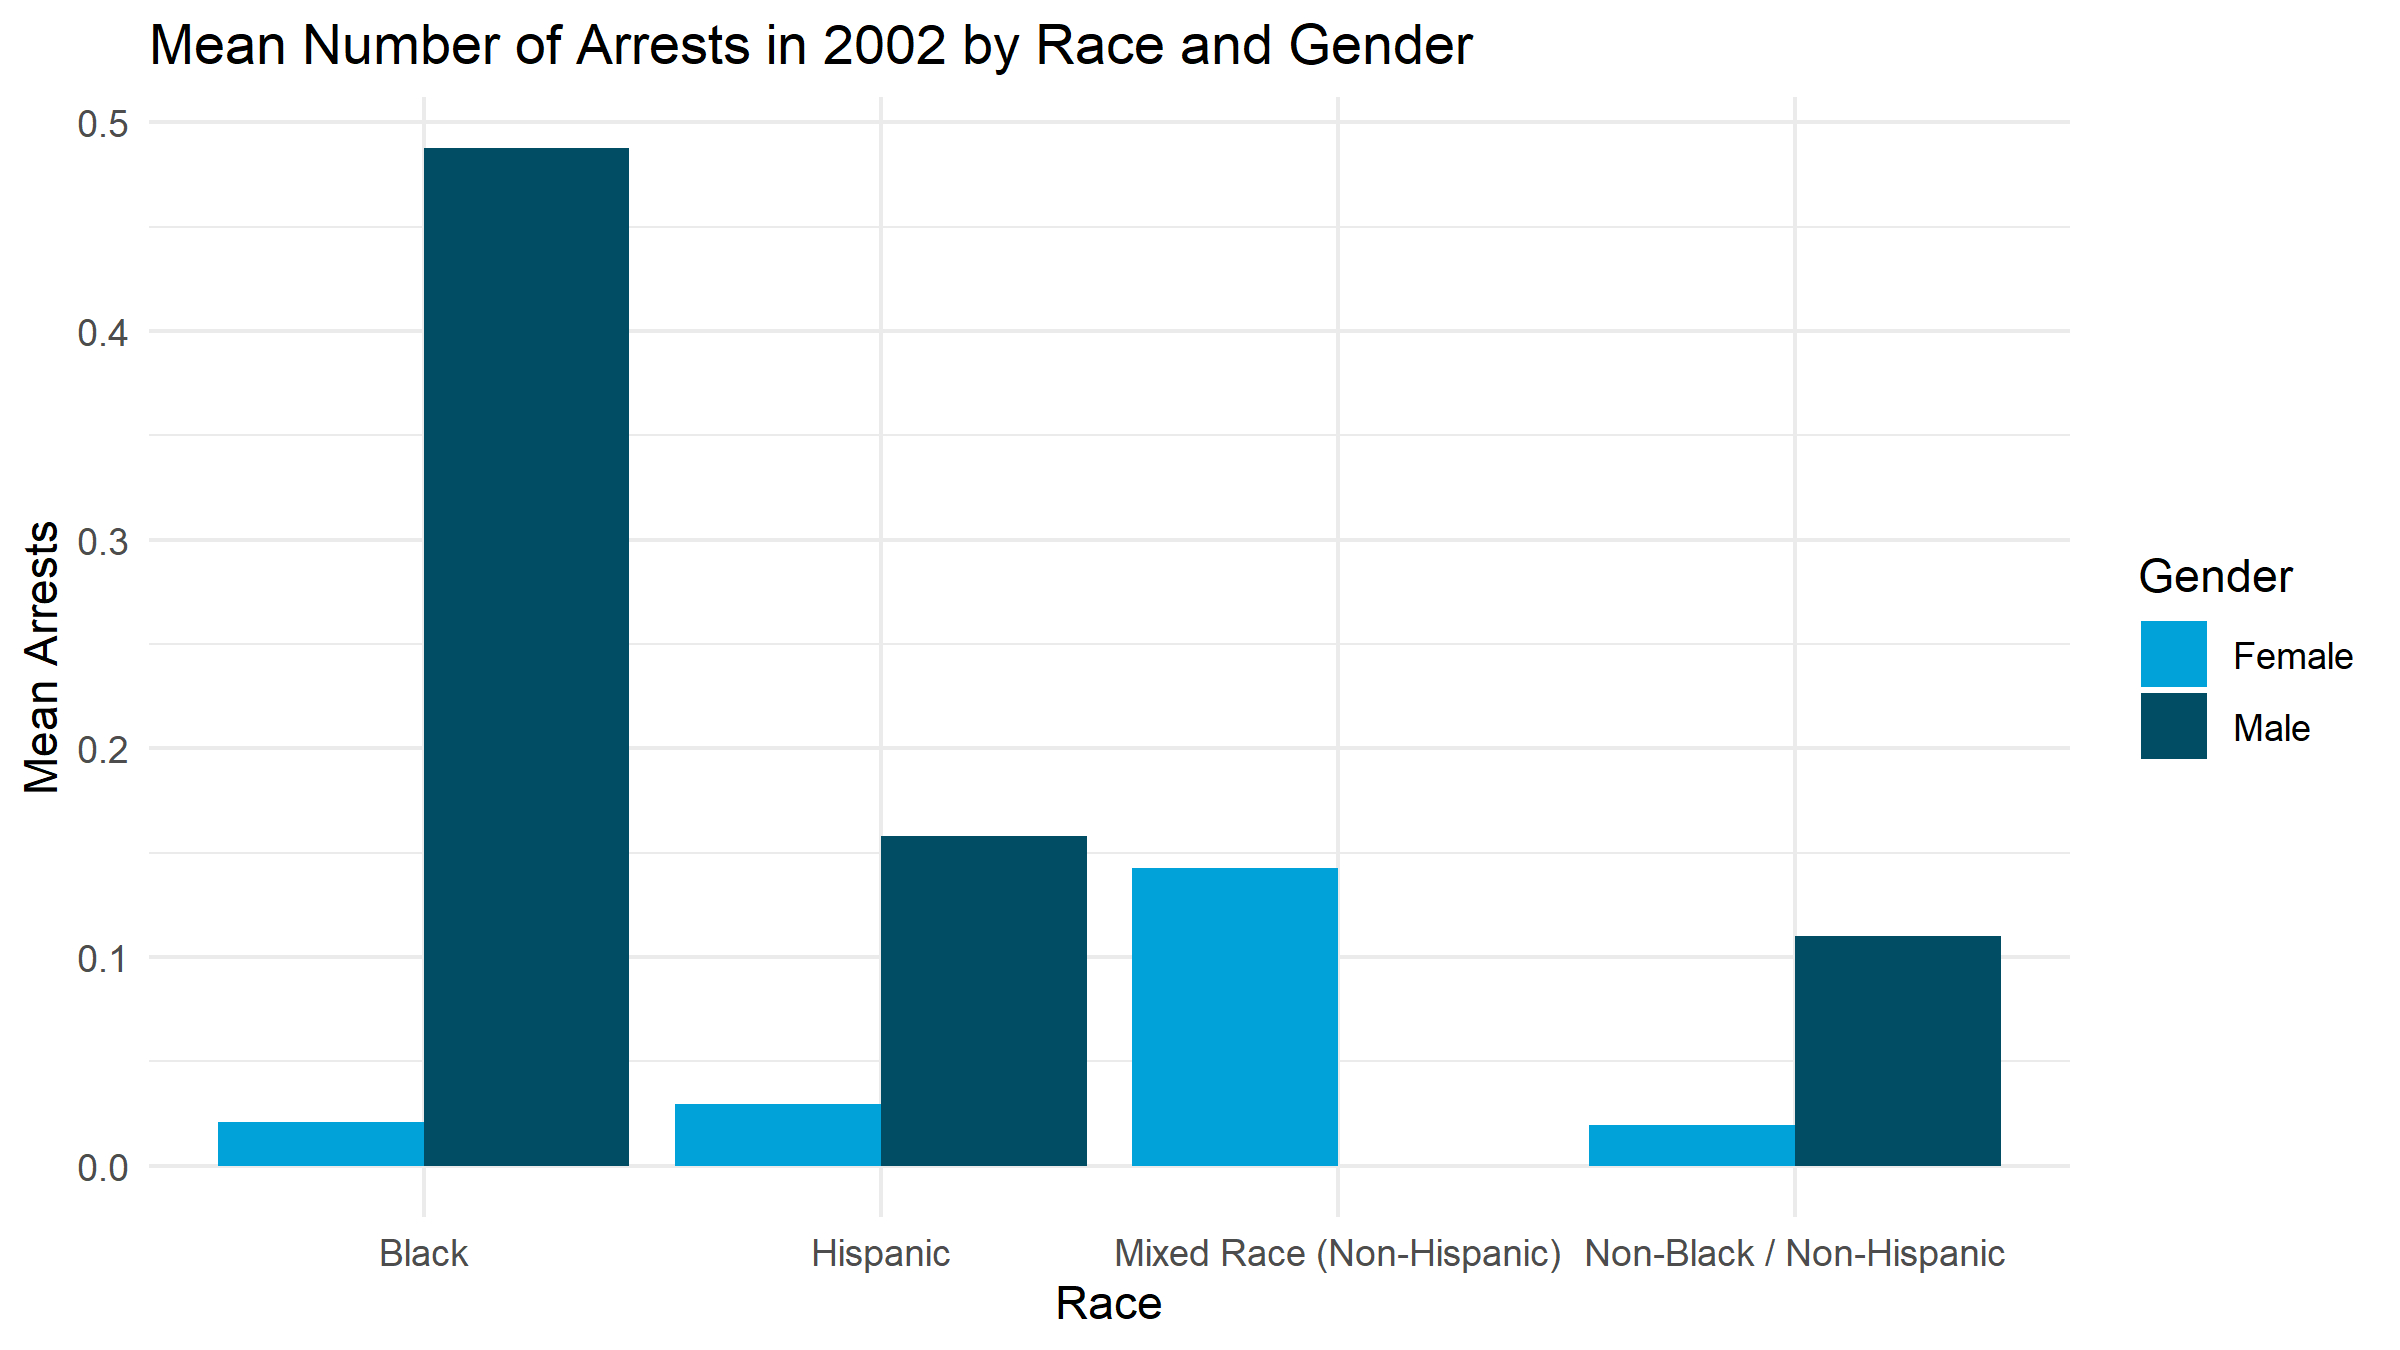
\includegraphics[width=.85\textwidth]{arrests_by_racegender}
    \end{center}
    \caption{Mean Number of Arrests in 2002 by Race and Gender}
    \label{fig:graph}
\end{figure}

This information is further presented in Table 1, where mean arrests are presented by race and gender. As mentioned, with the exception of the mixed race non-Hispanic category, male arrests are generally an order of magnitude larger than for their same demographic females. Black males had an average of .488 arrests in the year, while Hispanic and non-Black non-Hispanic groups had averages of .158 and .110, respectively. 

\begin{table}[H]

\caption{\label{tab:tab:summarystats}Mean arrests in 2002 by Race and Gender}
\centering
\begin{tabular}[t]{lrrrr}
\toprule
Gender & Black & Hispanic & Mixed Race Non Hispanic & Non Black Non Hispanic\\
\midrule
\cellcolor{gray!6}{Female} & \cellcolor{gray!6}{0.0211268} & \cellcolor{gray!6}{0.0298013} & \cellcolor{gray!6}{0.1428571} & \cellcolor{gray!6}{0.0193192}\\
Male & 0.4876712 & 0.1579509 & 0.0000000 & 0.1099476\\
\bottomrule
\end{tabular}
\end{table}


Table 2 shows the regression of mean arrests on the racial and gender categorical variables. Similar to the results indicated above, males had an average arrest .194 higher than females, and Black individuals had higher associated average arrests than Hispanic (.159 more average arrests), mixed race non-Hispanic (.174 more) and non-Black non-Hispanic (.189 more), holding all else fixed. 
 

% Table created by stargazer v.5.2.2 by Marek Hlavac, Harvard University. E-mail: hlavac at fas.harvard.edu
% Date and time: Thu, Feb 03, 2022 - 4:56:23 PM
\begin{table}[!htbp] \centering 
  \caption{Regression Output. Omitted category is Black Females.} 
  \label{tab:regression} 
\begin{tabular}{@{\extracolsep{5pt}}lc} 
\\[-1.8ex]\hline 
\hline \\[-1.8ex] 
 & \multicolumn{1}{c}{\textit{Dependent variable:}} \\ 
\cline{2-2} 
\\[-1.8ex] & Arrests in 2002 \\ 
\hline \\[-1.8ex] 
 Hispanic & $-$0.159$^{***}$ \\ 
  & (0.038) \\ 
  & \\ 
 Mixed Race (Non-Hispanic) & $-$0.174$^{**}$ \\ 
  & (0.083) \\ 
  & \\ 
 Non-Black / Non-Hispanic & $-$0.189$^{***}$ \\ 
  & (0.035) \\ 
  & \\ 
 Male & 0.194$^{***}$ \\ 
  & (0.022) \\ 
  & \\ 
 Constant & 0.155$^{***}$ \\ 
  & (0.026) \\ 
  & \\ 
\hline \\[-1.8ex] 
Observations & 8,621 \\ 
R$^{2}$ & 0.015 \\ 
Adjusted R$^{2}$ & 0.014 \\ 
Residual Std. Error & 1.019 (df = 8616) \\ 
F Statistic & 32.033$^{***}$ (df = 4; 8616) \\ 
\hline 
\hline \\[-1.8ex] 
\textit{Note:}  & \multicolumn{1}{r}{$^{*}$p$<$0.1; $^{**}$p$<$0.05; $^{***}$p$<$0.01} \\ 
\end{tabular} 
\end{table} 


\end{document}
